\documentclass[letterpaper,12pt]{article}

\usepackage[activeacute,spanish]{babel}
\usepackage[left=2cm,top=1cm,right=2cm, bottom=1cm,letterpaper, includeheadfoot]{geometry}

\usepackage{babel}
\usepackage[utf8]{inputenc}
\usepackage{algorithmic}
\usepackage{algorithm}
%\usepackage{enumitem}
\usepackage{enumerate}
\usepackage{multicol}
\usepackage{amssymb, amsmath, amsthm}
\usepackage{graphicx}
\usepackage{lmodern,url}
\usepackage{graphicx}
\usepackage{wrapfig}
\usepackage{hyperref}
\usepackage[dvipsnames]{xcolor}
\usepackage{color}

\floatname{algorithm}{Algoritmo}

\makeatletter


\usepackage{fancyhdr}
\pagestyle{fancy}
\fancypagestyle{plain}{%
    \fancyhf{}
    \lhead{\footnotesize\itshape\bfseries\rightmark}
    \rhead{\footnotesize\itshape\bfseries\leftmark}
    }

\setlength{\parindent}{1cm}


% macros
\newcommand{\cfbox}[2]{%
    \colorlet{currentcolor}{.}%
    {\color{#1}%
    \fbox{\color{currentcolor}#2}}%
}
\newcommand\myarrow{\mathrel{\overset{\makebox[0pt]{\mbox{\tiny def}}}{\Longleftrightarrow}}}
\newcommand{\grad}{\hspace{-2mm}$\phantom{a}^{\circ}$}
\newcommand{\Q}{\mathbb Q}
\newcommand{\R}{\mathbb R}
\newcommand{\N}{\mathbb N}
\newcommand{\Z}{\mathbb Z}
\newcommand{\C}{\mathbb C}
\newcommand{\U}{\mathcal U}
\newcommand{\ssi}{\Longleftrightarrow} %si y solo si
\newcommand{\To}{\Rightarrow}      %implica
\newcommand{\tq}{\mid }            % tal que
\newcommand{\exclusivo}{\veebar }  % o exclusivo
\renewcommand{\vec}[2]{\left(\begin{array}{c}{#1}\\{#2}\end{array}\right)}
\newcommand{\texii}[2]{\begin{minipage}{0.5\textwidth} #1 \end{minipage}  
                     \begin{minipage}{0.5\textwidth} #2 \end{minipage}}


%%%operadores matematicos
\providecommand{\abs}[1]{\lvert#1 \rvert}
\providecommand{\pin}[2]{\left< #1,#2 \right>} %producto interno
\providecommand{\dpartial}[2]{\frac{\partial #1}{\partial #2}} %derivada parcial


%Teoremas, Lemas, etc.
\theoremstyle{plain}
\newtheorem{teo}{Teorema}
\newtheorem{lem}{Lema}
\newtheorem{prop}{Proposici\'on}
\newtheorem{cor}{Corolario}
\newtheorem{prob}{Problema Controlable}
\newtheorem{nota}{Notaci\'on}
\newtheorem{obs}{Observaci\'on}
\hypersetup{%
    pdfborder = {0 0 0}
}

%%%%%%% inicio documento %%%%%%%
\begin{document}

%============Encabezado estandar============
\newpage
\pagestyle{fancy}
\fancyhf{}
\fancyhead[L]{\textit{Facultad de Ciencias Físicas y Matemáticas}}
\fancyhead[R]{\textit{Universidad de Chile}}
\fancyfoot[C]{\thepage} 

\begin{wrapfigure}{R}{0.2\textwidth} %this figure will be at the right
    \vspace{-5mm}
    
\includegraphics[width=0.2\textwidth]{img/fcfm2.png}
\end{wrapfigure}


\noindent
\textbf{MA1101-1 Introducción al Álgebra}\\
\textbf{Profesor: }Leonardo Sánchez C.\\
\textbf{Auxiliar: }Marcelo Navarro \\

\begin{center}
{\bf \Large Guia - Cardinalidad Conjuntos Infinitos}\\
\end{center}

\hspace{-1.65cm}
\fbox{\small \begin{minipage}{18.5cm} Resumen

\begin{multicols}{2}
\begin{itemize}
    \item $|A|=|B|$ si existe una función $f:A\to B$ biyectiva.
    
    \item $|A|\leq|B|$ si existe una función $f:A \to B$ inyectiva.
    
    \item $|A|<|B|$ si existe una función $f:A\to B$ inyectiva, pero no existe una función biyectiva $g:A \to B$
    
    \item Se tienen las siguientes propiedades:
        \begin{enumerate}
            \item $|A|\leq |A|$
            \item Si $A \subseteq B$, entonces $|A|\leq |B|$
            \item Si $|A|\leq |B|$ y $|B|\leq |C|$, entonces $|A|\leq |C|$
        \end{enumerate}
    
    \item \textbf{Teorema Cantor-Bernstein-Schöeder}
    $$|A|\leq |B| \land |B|\leq |A| \Rightarrow  |A|=|B|$$
    
    \item \textbf{Cardinal de la imagen de un conjunto}\\
    Si $f:A \to B$ es función, entonces $|f(A)|\leq |A|$
    
    \item $\N$ es infinito y si un conjunto $A$ cumple que $|A|=|\N|$, entonces se dirá que $A$ es numerable.
    Por otro lado si un conjunto $A$ cumple que $|A| \leq |\N|$ se dirá que $A$ es a lo más numerable.
    
    \item $|\N|$ es el menor cardinal infinito.
    
    \item Todo conjunto infinito $A$ inmediatamente cumple que $|A|\geq |\N|$. Es decir, $A$ es infinito si y sólo si $|A|\geq |\N|$.
    
    \item Sea $A$ un conjunto infinito tal que $|A|\leq |\N|$, entonces $A$ es numerable, es decir, $|A|=|\N|$
    
    \item Sea $A$ infinito y $B$ finito. Entonces $|A\cup B|=|A\setminus B|=|A|$
    
    \item $\Z$ y $\Q$ son numerables.
    
    \item Sea $A_1,A_2,\dots,A_n$ una colección finita de conjuntos numerables, entonces $\displaystyle \bigcup_{i=1}^{n}A_i$ también es numerable
    
    \item Sea $A_1,A_2,\dots,A_n$ una colección finita de conjuntos numerables, entonces $$\displaystyle \prod_{i=1}^{n}A_i= A_1 \times \cdots \times A_n$$ también es numerable.\\
        Una consecuencia de esto es que $\N^n , \Z^n$ y $\Q^n$ son numerables, con $n \in \N, ~ n\geq 1$
    
    \item Sea $(A_i)_{i\in \N}$ una colección numerable de conjuntos numerables, entonces $\displaystyle \bigcup_{i\in \N}A_i$ es numerable. 
    
    \item Sea $(A_i)_{i\in \mathcal{I}},~ \mathcal{I} \subseteq \N$, una colección a lo más numerable de conjuntos a lo más numerables (i.e. $|A_i|\leq |N|$). Entonces
    $\displaystyle \bigcup_{i\in \mathcal{I}}A_i$ es a lo más numerable (i.e. $\displaystyle |\bigcup_{i\in \mathcal{I}}A_i|\leq |\N|)$
    
    \item El producto de una familia numerable de conjuntos finitos de tamaño dos \emph{no es numerable}\\
    Ej: $\displaystyle \prod_{i \in \N} \{x_i,y_i\} ~ \text{ donde } x_i,y_i \in \R$ para todo $i \in \N$
    \item \textbf{Teorema Cantor}\\Sea $A$ un conjunto entonces $|A|<|\mathcal{P}(A)|$
    \item Un conjunto $A$ se dirá \emph{no numerable}  si $|\N|<|A|$
    \item $\R$, $\mathcal{P}(\N)$, $|(a,b)|$, $|(a,b]|$, $|[a,b)|$ y $|[a,b]|$    son \emph{no numerable}, con $a,b \in \R ~,a<b$ 


\end{itemize}
\end{multicols}
\end{minipage}}

\newpage 

\section{Algunas Estrategias Para Enfrentar Problemas.}
A continuación se presentarán algunas estrategias para enfrentar los problemas de cardinalidad para conjuntos infinitos (hay muchas otras formas de resolver los problemas)
\subsection{Conjuntos infinitos numerables}
Por lo general los problemas serán de probar que tal conjunto tiene la misma cardinalidad de los naturales, o probar que un conjunto tiene menor cardinalidad que otro, o probar que dado un conjunto $A$ que cumple alguna relación con otro conjunto $B$, probar que $B$ es numerable, etc.
Podemos realizar lo siguiente.
\begin{enumerate}[a)]
    \item \textbf{Mediante una inyección}\\
        Si se pide probar que $|A|\leq |B|$, independiente si son finitos, numerables o no numerables, si se encuentra una inyección de $A$ hacia $B$ se habrá probado lo pedido.
        
        
    \item \textbf{Mediante biyección}\\
        Si se pide probar que $|A|=|B|$, independiente si son finitos, numerables o no numerables, si se encuentra una biyección entre $A$ y $B$ se habrá probado lo pedido. Veamos el siguiente ejemplo.\\
        \textbf{[P2) i - Control 4 - 2014)]}\\
        Sean $A, B$ conjuntos no vacíos cualesquiera, demuestre que $|A\times B|=|B\times A|$\\
        En efecto, basta considerar la función $f: A\times B \to B\times A$ tal que $f(a,b)=(b,a)$. Esta función es biyectiva (Les dejo propuesto probarlo, de todas formas, pueden ver la pauta en nube mechona), entonces como encontré una función biyectiva entre $A\times B$ y $B\times A$ se tiene que $|A\times B|=|B\times A|$.
        
    \item \textbf{Mediante dos inyecciones}\\
        Si se pide probar que $|A|=|B|$, independiente si son finitos, numerables o no numerables, Si se encuentra una función $f:A \to B$ y otra función $g:B \to A$, ambas inyectivas, se tiene que $|A|\leq |B| \land |B|\leq|A|$ y por el \textbf{Teorema Cantor-Bernstein-Schöeder} se concluye que $|A|=|B|$. \\
        
        Un ejemplo de esto es el cardinal del continuo, es decir, $|2^{\N}|=|\R|=c$. Puede estudiarse en el propuesto 2 auxiliar 10. \href{https://www.u-cursos.cl/ingenieria/2017/1/MA1101/1/material_docente/}{\textcolor{BlueViolet}{\underline{Link a material docente}}}
        
    \newpage
        
    \item \textbf{Contradicción}\\
        La vieja confiable, también es independiente de si es finito, infinito numerable o no numerable. Habiendo tantas formas de realizar un problema de cardinalidad jamás he utilizado esto para atacar directamente un problema usando este método. Quizás lo combinaría con algún otro método. Sin embargo hay problemas que resultan directamente a partir de contradicción.\\
        
        \textbf{[Conjuntos finitos vs infinitos]}\\
        Demuestre que si $B \subseteq A$, $A$ es infinito y $B$ es finito, entonces $A \setminus B$ es infinito.\\
        
        En efecto, supongamos que $A \setminus B$ es finito. Trabajemos sobre el conjunto $A$...\\
        Podemos notar que $A=(A\setminus B)\cup B$. Con esto en cuenta, tneemos que A es igual a la unión de dos conjuntos finitos, pues por hipótesis de contradicción $A \setminus B$ es finito y por enunciado $B$ es finito. Entonces, como la unión de finitos es finito, se tiene que $A$ es finito, lo que es una contradicción pues por enunciado $A$ es infinito.\\
        
        Otro ejemplo lo pueden ver en la pregunta 5 auxiliar 10. \href{https://www.u-cursos.cl/ingenieria/2017/1/MA1101/1/material_docente/}{\textcolor{BlueViolet}{\underline{Link a material docente}}}
        
        \newpage
    \item \textbf{Escribir el conjunto como unión (a lo más numerable) de conjuntos}\\
        Dado un conjunto $A$, si nosotros sabemos que $A$ es numerable podemos representarlo como una \textbf{colección infinita de elementos enumerados/enlistados}, es decir, $A=\{a_1,a_2,\dots, a_n,\dots \}$ De esta forma podemos escribir el conjunto $A$ como
        $$\displaystyle A=\bigcup_{i\in \N} \{a_i\}$$
    
        Es directo de la igualdad de conjuntos que $\displaystyle |\bigcup_{i\in \N} \{a_i\}|= |A| =|\N|$ (lo ultimo pues supusimos que $A$ es numerable).\\
        Sin embargo, nosotros queremos obtener otro resultado a partir de esto, el cual es el siguiente.\\
        Como se tiene que $\displaystyle A=\bigcup_{i\in \N} \{a_i\}$, en el lado derecho de la igualdad tenemos ante nosotros que $\displaystyle \bigcup_{i\in \N} \{a_i\}$ es una unión numerable de conjuntos a lo más numerables, por lo tanto $\displaystyle |\bigcup_{i\in \N} \{a_i\}|\leq |\N|$ (Ver resumen, columna derecha).
        Este resultado nos ayudará mucho, veamos el siguiente ejemplo.\\
    
        \textbf{[P2) b.1 - Control 4 - 2016)]}\\ Sea $g:E \to F$, una función. Pruebe que si $|E|=|\N|$, entonces $|g(E)|\leq|\N|$
        \begin{itemize}
            \item En efecto, como $E$ es numerable, entonces podemos escribir $E$ como una colección infinita de elementos.\\
        $\Longrightarrow E=\{e_0,e_1,e_2, \dots, e_k, \dots \}$, por otro lado, tenemos que $g(E)$ al ser un conjunto imagen, lo podemos representar como $\displaystyle g(E)=\{ g(e) : e\in E\}=\bigcup_{e \in E}\{g(e)\}$. Luego como habíamos dicho que $E=\{e_0,e_1,e_2, \dots, e_k, \dots \}$ se tiene que\\
        $$\displaystyle  g(E)=\bigcup_{e \in E}\{g(e)\}=\bigcup_{i\in \N}\{g(e_i)\}$$
        Luego $g(E)$ es igual a una unión numerable de singletons (los singletons son a lo más numerables pues son finitos), entonces se tiene que $\displaystyle |g(E)|=|\bigcup_{i\in \N}\{g(e_i)\}| \leq |\N|$. Por lo tanto $|g(E)|\leq |\N|$ \\
    
        \textit{obs: en la desigualdad $|\displaystyle \bigcup_{i\in \N}\{g(e_i)\}| \leq |\N|$ se ocupo lo planteado anteriormente. pues es la unión numerable de conjuntos a lo más numerables}
        
        \end{itemize}
        
        Puede ver otro ejemplo de esto en la pregunta 4 auxiliar 10. \href{https://www.u-cursos.cl/ingenieria/2017/1/MA1101/1/material_docente/}{\textcolor{BlueViolet}{\underline{Link a material docente}}}
        \newpage
        
    \item \textbf{Probar que un conjunto es infinito + función inyectiva}
    
    Si se desea probar que un conjunto $A$ es numerable, es decir que $|A|=|\N|$. Una buena forma es dividir el problema en dos partes
    
    \begin{enumerate}
        \item Determinar que $A$ es infinito, con esto se tiene que $|A|\geq |\N|$
        \item Encontrar una función $f:A \to \N$ inyectiva, de esta forma $|A|\leq |\N|$
    \end{enumerate}
    Luego basta con concluir con el \textbf{Teorema Cantor-Bernstein-Schöeder} que $|A|=|\N|$. Veamos el siguiente ejemplo.
    
    \textbf{[P2) b - Control 4 - 2015)]}\\ Se define $M=\{A\subseteq \Q: |A|=2 \}$. Demuestre que $M$ es numerable.
        \begin{itemize}
            \item En efecto, veamos primero que $M$ es infinito. Los elementos que viven en $M$ son los conjuntos de dos elementos, que son subconjuntos de $\Q$, es decir, sea $p,q \in Q, p\neq q,$ entonces  $\{p,q\}\in M$, de forma general, $M=\{\{p,q\} : p,q \in \Q \land p\neq q \}$
            Podemos tomar el conjunto $M_{p=0}=\{\{0,q\} : q \in \Q \land 0\neq q \} $, luego $q$ puede tomar infinitos valores, ya que $q\in \Q$ y $\Q$ es infinito, entonces las parejas de la forma $\{0,q\}$ son infinitas.\\
            Ahora notamos que $M_{p=0} \subseteq M$ esto pues las parejas de la forma $\{0,q\}$ son un caso puntual de las parejas $\{p,q\}$. Por lo tanto $M$ debe ser infinito y con ello
             \begin{alignat}{2}
                && |M|&\geq|\N|
             \end{alignat}
            
            Por otro lado, podemos definir la siguiente función $\varphi: M \to \Q \times \Q$ que cumple que $\varphi(\{p,q\})=(min\{p,q\},max\{p,q\})$. \\
            Por ejemplo: $\varphi(\{5,2\})=(min\{5,2\},max\{5,2\})=(2,5)$ pues $2<5$.\\[5mm]
            Probemos que $\varphi$ es inyectiva.\\
            En efecto, sea $\{p_1,q_1\}, \{p_2,q_2\} \in M$ tal que $\varphi(\{p_1,q_1\})=\varphi(\{p_2,q_2\} ) $. Sin perdida de generalidad, podemos suponer que 
            \begin{itemize}
                \item $min\{p_1,q_1\}=p_1 ~~~~~ \land ~~~~~ max\{p_1,q_1\}=q_1$
                \item $min\{p_2,q_2\}=p_2 ~~~~~ \land ~~~~~ max\{p_2,q_2\}=q_2$
            \end{itemize}
            Pues en cualquier otro caso, podemos cambiar roles usando que $\{p_1,q_1\}=\{q_1,p_1 \}$ ya que estamos hablando de conjuntos (y solo me interesa que elementos hay, no el orden). Entonces 
             \begin{alignat}{2}
                &\Longrightarrow\quad &\varphi(\{p_1,q_1\})  &= \varphi(\{p_2,q_2\})\notag\\ 
                &\myarrow  &(min\{p_1,q_1\},max\{p_1,q_1\}) &= (min\{p_2,q_2\},max\{p_2,q_2\})\notag\\  
                &\Longrightarrow & (p_1,q_1) &= (p_2,q_2) \notag\\
                &\Longrightarrow &p_1=p_2 & \land  q_1=q_2 \notag\\
                &\Longrightarrow & \{p_1,q_1\} &=\{p_2,q_2\} \notag
            \end{alignat}
            Por lo tanto $\varphi : M \to \Q \times \Q$ es inyectiva entonces 
             \begin{alignat}{1}
                 |M|\leq|\Q \times \Q|=|\Q^{2}|=|\N|
             \end{alignat}
             Donde se uso que producto finito de numerables, es numerable.\\ Finalmente por (1) y (2), usando el \textbf{Teorema Cantor-Bernstein-Schöeder} se tiene que $|M|=|\N|$, por lo tanto $M$ es numerable.
        \end{itemize}
        
    
    \item \textbf{Probar que un conjunto es infinito + inclusión}\\
    Supongamos que tenemos un conjunto $B$ numerable, y se desea probar que un conjunto $A$, que guarda una relación con $B$, es numerable. Una buena forma es dividir el problema en dos partes
    \begin{enumerate}
        \item Determinar que $A$ es infinito, con esto se tiene que $|A|\geq |\N|$ (por lo tanto $A$ es numerable)
        \item Ver que $A\subseteq B^{k}$ con $k\in \N, ~ k\geq 1$, de esta forma $|A|\leq |B^{k}|=|B|=|\N|$
    \end{enumerate}
    Luego basta con concluir con el \textbf{Teorema Cantor-Bernstein-Schöeder} que $|A|=|\N|$. Veamos el siguiente ejemplo.\\[2mm]
    \textbf{Conjuntos de los primos:}\\
    Demuestre que el conjunto de los números primos $\mathbb{P}$ es numerable, es decir, $| \mathbb{P}|=|\N|$
    \begin{itemize}
        \item En efecto, es claro que $\mathbb{P}\subseteq \N$, entonces $|\mathbb{P}|\leq |\N|$\\
    Veamos ahora que $\mathbb{P}$ es infinito. Procedamos por contradicción, supongamos que $\mathbb{P}$ es finito, entonces $\mathbb{P}=\{p_1,p_2,\dots,p_{n}\}$ con $p_1<p_2<\dots<p_n$. Construyamos el número $Q=p_1\cdot p_2\cdot ... \cdot p_n +1$, es directo que $Q$ es \textbf{estrictamente mayor} que cualquier elemento de $\mathbb{P}$ (pues los primos son positivos y $Q$ lo construi mediante multiplicaciones). Si logramos demostrar que $Q$ es primo, habremos encontrado un número primo que no esta en $\mathbb{P}$ rompiendo la idea de que los primos son finitos.\\
    En efecto, por contradicción, supongamos que $Q$ es compuesto, por el teorema fundamental del álgebra $Q$ es primo o debe ser producto de números primos. Como supusimos que es compuesto, $Q$ debe ser producto de números primos. Luego debe existir un primo $ p_j \in \mathbb{P}$ que divide a $Q$, además $p_j$ debe dividir a $p_1\cdot p_2\cdot ... \cdot p_n$ pues participa en la multiplicación (ej: $2$ divide a $2\times3\times11$) \\[5mm]
    
    Que $p_j$ divida a $Q$ significa que $\exists k\in \Z,~ Q=p_j\cdot k$\\
    Que $p_j$ divida a $p_1\cdot p_2\cdot ... \cdot p_n$ significa que $\exists k'\in \Z,~ p_1\cdot p_2\cdot ... \cdot p_n =p_j\cdot k'$\\[5mm]
    Ahora como sabemos que $Q=p_j\cdot k$ y $p_1\cdot p_2\cdot ... \cdot p_n =p_j\cdot k'$, restando ambas igualdades y usando que $Q=p_1\cdot p_2\cdot ... \cdot p_n +1$ obtenemos que:
    
            \begin{alignat}{2}
                &\Longrightarrow\quad &Q-p_1\cdot p_2\cdot ... \cdot p_n  &= p_j \cdot k - p_j \cdot k'\notag\\ 
                &\Longleftrightarrow & (p_1\cdot p_2\cdot ... \cdot p_n +1) - p_1\cdot p_2\cdot ... \cdot p_n&=  p_j \cdot (k - k')\notag\\  
                &\Longrightarrow & 1 &= p_j \cdot k'' ~~~~~ k'' \in \Z\notag
            \end{alignat}

    Es decir, $p_j$ divide a $1$!!!!!!! CHAN CHAN!. Esto es genial, pues el unico número que divide a 1 es el mismo 1, por lo tanto $p_j=1$ y contradice el hecho de que sea primo. por lo tanto $Q$ NO PUEDE SER COMPUESTO.\\
    
    Luego Q es primo, y es estrictamente mayor que cualquier elemento de $\mathbb{P}$, por lo tanto encontre un nuevo número primo que no estaba en el conjunto finito de los primos que asumimos. Lo que contradice que los números primos sean finitos.\\
    Por lo tanto los primos son infinitos! es decir $|\mathbb{P}|\geq |\N|$. Y por el \textbf{Teorema Cantor-Bernstein-Schöeder} se concluye que los primos son numerables.
    \end{itemize}
    
    Pueden ver otro ejemplo de esto en la pregunta 4 auxiliar 10. \href{https://www.u-cursos.cl/ingenieria/2017/1/MA1101/1/material_docente/}{\textcolor{BlueViolet}{\underline{Link a material docente}}}
    
    
    \subsection{Conjuntos infinitos no numerables}
    Las siguientes estrategias son una particularidad de las formas a,b,c y d, de las estrategias de la sección anterior.
    \begin{enumerate}[a)]
        \item \textbf{biyección con un conjunto no numerable}\\
        Si se pide demostrar que un conjunto $A$ es no numerable, basta con encontrar una biyección entre el conjunto $A$ con algún conjunto no numerable (ver resumen, columna derecha)\\
        
        \textbf{Funciones trigonométricas}\\
        \begin{itemize}
            \item  Demuestre que $|(-\frac{\pi}{2},\frac{\pi}{2})|$ es no numerable.\\
        En efecto, basta considerar la función tangente, $tg :(-\frac{\pi}{2},\frac{\pi}{2})\to \R$, que sabemos que es biyectiva por Introducción al Calculo. Por lo tanto $|(-\frac{\pi}{2},\frac{\pi}{2})|=|\R|$
        \end{itemize}
        
        \item \textbf{inyección desde un no numerable al conjunto que queremos}\\
        Si nos piden demostrar que $|A|$ es no numerable, basta con que encontremos una inyección desde $B$ hacia $A$, donde $B$ es no numerable, con esto habremos demostrado que $|B|\leq|A|$ y como $B$ es no numerable se tiene que $|\N|<|B|\leq|A|$, luego $A$ es no numerable. \\
        
        Un ejemplo de esto es la pregunta 6 auxiliar 10. \href{https://www.u-cursos.cl/ingenieria/2017/1/MA1101/1/material_docente/}{\textcolor{BlueViolet}{\underline{Link a material docente}}}
        
    \end{enumerate}
    
    \newpage
    

    \section{Problemas}
    
    \begin{enumerate}[\bf P1.]
        \item \textbf{[Control 2 - 2005]} Sea $\mathcal{G}$ el conjunto de todas las circunferencias en el plano cartesiano cuyos centros tienen coordenadas racionales y su radio es racional, es decir $C \in \mathcal{G} \Leftrightarrow  C$ es una circunferencia de centro $(a, b)$ y radio $r$ con $a, b, r \in \Q$. Pruebe que el conjunto de todos los pares de puntos $(P, Q)$ donde $P$ y $Q$ son los extremos de los diámetros horizontales de las circunferencias de $\mathcal{G}$, es infinito numerable.
        
        \hyperlink{page.12}{\cfbox{Maroon}{\bf Solución P1}}\vspace{3mm}
        
        \item \textbf{[Control 2 - 2003]}\begin{enumerate}
            \item Pruebe que el conjunto de todas las rectas no verticales que pasan por el punto $(0, 1)$ es no numerable.
            \item Pruebe que el conjunto de todas las rectas no verticales que pasan por el punto $(0, 1)$ y cortan al eje $OX$ en una coordenada racional, es numerable.
            \item Pruebe que el conjunto de todas las rectas no verticales, que no pasan por el origen y tales que cortan a los ejes $OX$ y $OY$ en coordenadas racionales, es numerable. 
        \end{enumerate}
        \hyperlink{page.13}{\cfbox{Maroon}{\bf Solución P2}}\vspace{3mm}
        
        \item \textbf{[Control 2 - 2001 \& Control 4 - 2016]} Para todo $n \in \N$ se tiene una función $f_n:\R \to \R$. Además, $f_1=id_{\R}$. Sea $A\subseteq \R$ y $B=\{f_n(a): a \in A, n \in \N \}$. Pruebe que si $A$ es infinito numerable, entonces B es infinito numerable.
        
        \hyperlink{page.13}{\cfbox{Maroon}{\bf Solución P3}}\vspace{3mm}
        
        \item \textbf{[c3 - 1996]} Sea $A=\{\frac{p}{q} :  (\exists n \in \N, q=2^{n}) \land (p\in \N, p<q)\}$. Probar que $A$ es infinito numerable
        
        \hyperlink{page.14}{\cfbox{Maroon}{\bf Solución P4}}\vspace{3mm}
        
        \item Muestre que el conjunto
        $$A=\{(m,n)\in \Z \times \Z : m\leq n \} \text{ es infinito numerable } $$
        
        \hyperlink{page.14}{\cfbox{Maroon}{\bf Solución P5}}\vspace{3mm}
        
        \item Sean $C,D$ conjuntos no vacíos, con $C$ finito y $D$ infinito numerable.\\
        Sea $$\mathcal{F}(C,D)=\{f:C\to D ~|~ f \text{ es función } \}$$
        Muestre que $\mathcal{F}(C,D)$ es infinito numerable.\\
        \textbf{Indicación: }Recuerde que significa $A^{B}$ donde $A,B$ son conjuntos.
        
        \hyperlink{page.14}{\cfbox{Maroon}{\bf Solución P6}}\vspace{3mm}
        
        \item Sea $B$ un conjunto numerable y $\preceq$ una relación de orden total definida en $B$ (recuerde que $\preceq$ es de orden total si y sólo si, $\forall a,b \in B$ se tiene que $a \preceq b \lor b\preceq a$). Pruebe que dado $a\in B$, uno de los dos conjuntos siguientes es infinito numerable.
        $$ B_1=\{b\in B : b\preceq a \}, B_2=\{b\in B : a\preceq b \} $$
        
        \hyperlink{page.14}{\cfbox{Maroon}{\bf Solución P7}}\vspace{3mm}
        
        \item Sea $\displaystyle E=\{(a_1,a_2,\dots,a_n) \in \{-1,1\}^{n} ~|~ n\in \N, n\geq 2, \sum_{i=1}^{n}a_i=0. \}$. Es decir,
        $$\displaystyle a=(a_1,\dots,a_n) \in E \Longleftrightarrow  a_1,\dots,a_n \in \{-1,1 \}, \text{ tales que } \sum_{i=1}^{n}a_i=0.  $$
        \begin{enumerate}
            \item Muestre que $E$ es infinito.
            \item Pruebe que $E$ tiene la misma cardinalidad de $\N$
        \end{enumerate}
        
        \hyperlink{page.14}{\cfbox{Maroon}{\bf Solución P8}}\vspace{3mm}
        
        \item Sea $A=\{x\in \R : \exists k \in \Z. \exists i \in \N, x=\frac{k}{3^{i}} \}.$ Pruebe que $A$ es numerable
        
        \hyperlink{page.14}{\cfbox{Maroon}{\bf Solución P9}}\vspace{3mm}
        
        \item \textbf{[C2 - 2010-2 - Varas]} Se definen $M_k=\{ A\subseteq \N: |A|=k\}$ y $M=\{A\subseteq \N: |A|< \infty \}$
        \begin{enumerate}
            \item Muestre que para todo $k \in \N \setminus \{0\}$, $M_k$ es un conjunto infinito.
            \item Describa $M_1$ y muestre que $|M_1|=|\N|$ indicando la biyección.
            \item Describa $M_2$ y muestre que $|M_2|\leq|\N^{2}|$, concluya que $M_2$ es numerable.
            \item Muestre que $|M_k|\leq |\N^{k}|$, concluya que $M_k$ es numerable.
            \item Utilice lo anterior para determinar la cardinalidad del conjunto $M$
        \end{enumerate}
        
        \hyperlink{page.14}{\cfbox{Maroon}{\bf Solución P10}}\vspace{3mm}
        
        
        \item Demuestre que $C=\{x \in [0,+\infty)~|~ \exists n \in \N \setminus \{0 \}, x^{n} \in \N \}$ es numerable.
        
        \hyperlink{page.14}{\cfbox{Maroon}{\bf Solución P11}}\vspace{3mm}
        
        \item Demuestre que $E=\{x=(x_1,x_2,x_3) \in \R\times \N \times \N~|~ \exists n \in \N, x_1+x_2+x_3=n \}$ Es numerable.
        
        \hyperlink{page.14}{\cfbox{Maroon}{\bf Solución P12}}\vspace{3mm}
        
        \item \textbf{[Apunte 2017]} Demuestre que los siguientes conjuntos son no numerables.
            \begin{enumerate}
                \item $A=\{x\in \R^{3} : \exists n \in \N, x_1+x_2+x_3=n \}$
                \item $\mathcal{T}=\{T \subseteq \R^{2} : T \text{ es un triángulo } \}$
            \end{enumerate}
            
            \hyperlink{page.14}{\cfbox{Maroon}{\bf Solución P13}}\vspace{3mm}
            
        \item \textbf{[Painequeo]} Sea $X\subseteq \R$ numerable, Se define $-X=\{-x: x\in X\}$. Demuestre que el conjunto $X\cup -X$ es numerable.
        
        \hyperlink{page.15}{\cfbox{Maroon}{\bf Solución P14}}\vspace{3mm}
        
        \item Sea $A\subseteq \R$ el conjunto 
        $$A=\{r+s\sqrt{2}: r,s\in \Q \}  $$
        Pruebe que $A$ es infinito numerable
        
        \hyperlink{page.16}{\cfbox{Maroon}{\bf Solución P15}}\vspace{3mm}
        
        \item Si $A$ y $B$ con conjuntos infinitos numerables. Pruebe que $A\times B$ es numerable. Para esto defina $H_b=\{ (a,b) : a\in A\}$ con $b \in B$ fijo y escriba adecuadamente $A\times B$.
        
        \hyperlink{page.16}{\cfbox{Maroon}{\bf Solución P16}}\vspace{3mm}
        
        \item Sea $H=\{ a^{b} ~|~ a \in \N \setminus \{0\} \land b\in \Q\}$. Pruebe que $H$ es numerable.
        
        \hyperlink{page.16}{\cfbox{Maroon}{\bf Solución P17}}\vspace{3mm}
        
        \item Considere el conjunto $C=\{\dots, -16,-9,-4,-1,0,1,4,9,16,\dots \}$. Pruebe que $C$ es numerable.
        
        \hyperlink{page.16}{\cfbox{Maroon}{\bf Solución P18}}\vspace{3mm}
        
        \item Sea $C=\{(m,n)\in \Q\times \Z : (m+n) \in \N \}$. Demuestre que $C$ es numerable.
        
        \hyperlink{page.16}{\cfbox{Maroon}{\bf Solución P19}}\vspace{3mm}
        
        \item Sea $A$ un conjunto y $f: A \to \N$ una función. Demuestre que si $\forall n \in \N, f^{-1}(\{n\})$ es numerable, entonces $A$ es numerable.
        
        \hyperlink{page.16}{\cfbox{Maroon}{\bf Solución P20}}\vspace{3mm}
        
        \item \textbf{[C4 - 2014]} Se define el conjunto $\mathcal{F}$ por
        $$ \mathcal{F}=\{ f:\N \to \N~|~ f(0)=0 \land \exists d\in \N, \forall n \in \N, f(n+1)=f(n)+d \} $$
        Demuestre que $\mathcal{F}$ es numerable
        
        \hyperlink{page.17}{\cfbox{Maroon}{\bf Solución P21}}\vspace{3mm}
        
        \item Sea $A=\{ (m^4+5)^{n}: m,n\in \N \}$. Demuestre que $A$ es infinito numerable.
        
        \hyperlink{page.18}{\cfbox{Maroon}{\bf Solución P22}}\vspace{3mm}
        
        \item Sea $A,B,C$ conjuntos tal que $|A|<|B|$ y $B\subseteq C$. Demuestre que $|A|<|C|$.
        
        \hyperlink{page.18}{\cfbox{Maroon}{\bf Solución P23}}\vspace{3mm}
        
        \item \textbf{[Desafio]}Un polinomio de se define como una función $P$ de la forma $P(x)=p_0+p_1x+p_2x^2+\dots+p_nx^{n} $ (notar que la suma es finita).
        Además diremos que dos polinomio $P$ y $Q$ son iguales si los coeficientes $p_k$ y $q_k$ son iguales para todo $k$. Además diremos que el grado de un polinomio $P$ es el natural $k$ más grande en donde $p_k\neq0$\\
        Demuestre que el conjunto $\Z[x]$ de todos los polinomios con coeficientes enteros es numerable.\\
        Para esto siga los siguientes pasos:
        \begin{itemize}
            \item Defina el conjunto $P_n$ como todos los polinomios de grado $n$ y construya una función inyectiva $f$ desde $\Z^{i}$ hasta $P_n$ con un $i\in \N$ adecuado.
            \item Escriba $\Z[x]$ en términos de $P_n$ y concluya.
        \end{itemize}
        
        \hyperlink{page.18}{\cfbox{Maroon}{\bf Solución P24}}\vspace{3mm}
        
        \newpage
        \item \textbf{[Desafio 2]} Un numero real se llamará \emph{algebraico} si es solución de 
        $$ a_nx^{n}+\dots+a_1x+a_0=0 $$
        donde $n\in \N$, $\forall i\in \{0,\dots, n\}, a_i \in \Z$ y $a_n\neq 0$. Además diremos que si un número no es algebraico entonces lo llamaremos \emph{trascendente}.
        En este pregunta usted demostrará que el conjunto de todos los números algebraicos $A$ es numerable y el conjunto de todos los números trascendentes $T$ es no numerable. Para esto, siga los siguientes pasos
        \begin{enumerate}
            \item Resuelva la pregunta anterior o simplemente use el resultado.
            \item Escriba $A$ en términos de un polinomio.
            \item Defina $A_k$ como el conjunto de números algebraicos obtenidos a partir de los polinomios de grado $k$, y use esto para demostrar que $A$ es numerable.
            \item Estudie la relación que hay entre $A, T$ y $\R$ y concluya que $T$ es no numerable.
        \end{enumerate}
        
        \hyperlink{page.18}{\cfbox{Maroon}{\bf Solución P25}}\vspace{3mm}
        
        
    \end{enumerate}
    
    \newpage 
    
    \section{Soluciones}
    \begin{enumerate}[\bf P1.]
        \item Veamos primero como se puede escribir el conjunto de todos los pares de puntos $(P,Q)$ donde $P$ y $Q$ son extremos de los diámetros horizontales, el cual llamaremos $E$. Para esto veamos la siguiente imagen que representa a una circunferencia en un lugar arbitrario del plano cartesiano.
        \begin{figure}[H]
            \centering
            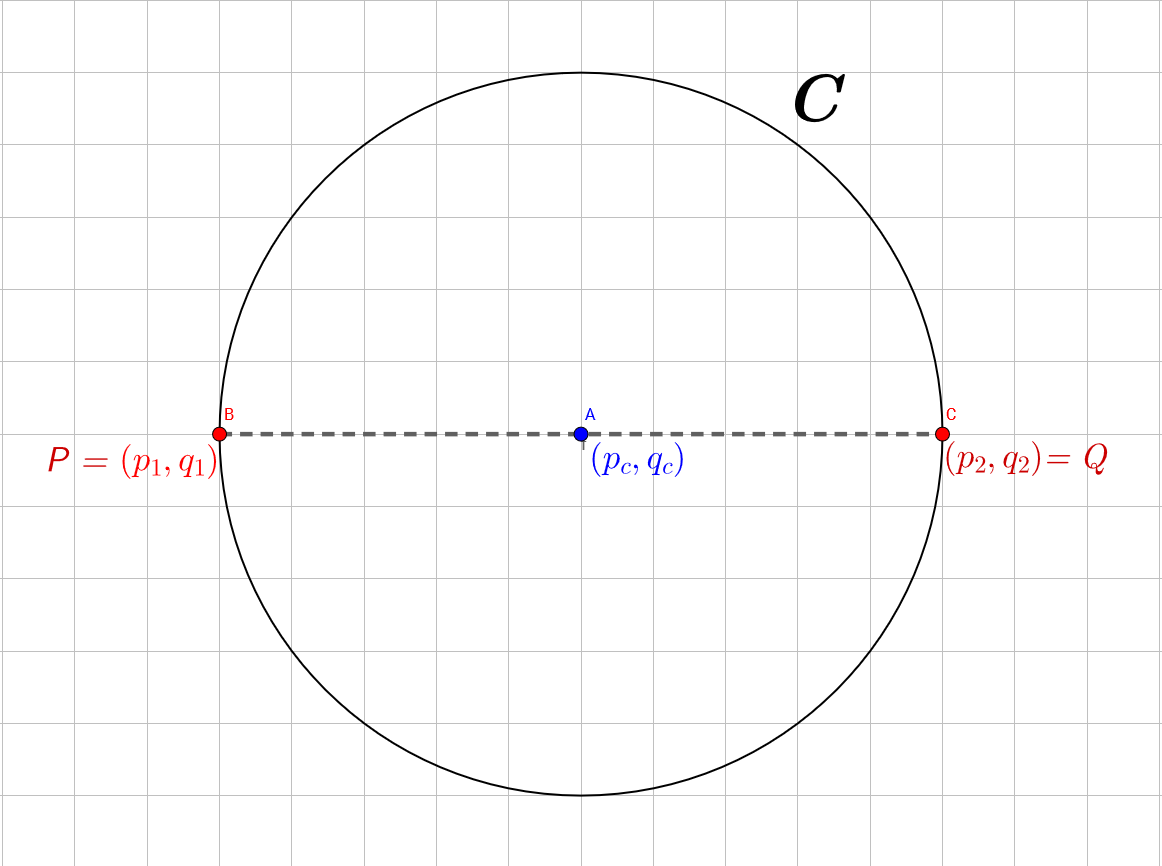
\includegraphics[scale=0.3]{img/p1.png}
            \caption{Ejemplo de Circunferencia \textbf{$C$}.}
            \label{fig:p1}
        \end{figure}
        El segmento punteado es el diámetro horizontal de esta circunferencia, donde el punto $P=(p_1,q_1)$ y $Q=(p_2,q_2)$ son los puntos que definen el diámetro. En este caso el par $(P,Q)$ pertenece al conjunto $E$, notemos que de aqui podemos establecer las propiedades que deben cumplir las coordenadas de $P$ y de $Q$.\\
        En primar lugar, las coordenadas $y$ son iguales (ya que estoy hablando de un diámetro horizontal). Además sin perdida de generalidad podemos decir que la primera coordenada de $P$ debe ser menor que la primera coordenada de $Q$, pues $P$ se ubica a la izquierda de $Q$ en el plano.\\
        Luego el conjunto estudiadio se puede escribir por compresión de la siguiente manera
        $$ E=\{(P,Q) ~|~ P=(p_1,q_1),Q=(p_2,q_2), (p_1<p_2) \land (q_1=q_2),~ p_1,q_1,p_2,q_2 \in \Q  \} $$
        De aqui podemos reducir las condiciones que se deben cumplir, obteniendo el siguiente conjunto
        $$ E=\{(P_{(p_1,q_h)},Q_{(p_2,q_h)} ~|~ p_1<p_2,~ p_1,p_2,q_h \in \Q \} $$
        Donde $q_h$ viene a reemplazar el valor de las coordenadas $y$ que tenian el mismo valor para $P$ y $Q$.
        Notemos que el radio de estas circunferencias será de la forma $r=\frac{p_2-p_1}{2}$ y el centro será $(\frac{p_1+p_2}{2},q_h)$.\\
        Finalmente, Nos falta demostrar que es infinito numerable.\\
        En efecto, $E$ es infinito pues puedo dejar fijo $p_1=0$, $q_h=0$ y $p_2$ puede recorrer todo $(\Q_{+}\setminus\{ 0\})$, por lo tanto $E$ es infinito, entonces $|E|\geq |\N|$.\newpage
        Por otro lado, En el conjunto $E$ estoy guardando una colección de pares ordenados, pues tengo elementos de la forma $(P,Q)$ que realmente es un \emph{objeto} que almacena dos puntos de un plano que viven en $\Q \times \Q$, es decir, $E\subseteq  \Q \times \Q$, entonces $|E|\leq |\Q \times \Q|=|\N|$.\\[2mm]
        Finalmente por \textbf{Teorema Cantor-Bernstein-Schöeder} se tiene que $|E|=|\N|$, por lo que $E$ es numerable.\\
        
        Puede ver otra forma de resolver esto en los siguientes links\\
        \href{https://drive.google.com/drive/folders/0B2BWTqIXpSJsakxLVUNxejQyc1U}{\textcolor{BlueViolet}{\underline{Nube Mechona - C2 2005}}}\\
        \href{https://www.u-cursos.cl/ingenieria/2016/1/MA1101/5/material_docente/}{\textcolor{BlueViolet}{\underline{P3 - Pauta auxiliar 8 : MA1101-5 - Otoño - 2016}}}\\
        
        \item Puede ver la respuesta en \href{https://drive.google.com/drive/folders/0B2BWTqIXpSJsakxLVUNxejQyc1U}{\textcolor{BlueViolet}{\underline{Nube Mechona - C2 2003}}}\\
        
        \item \textit{Recuerdo: el conjunto imagen se define como $f(A)=\{f(x) : x\in A \}$}\\
        Veamos que $B$ es infinito. Notemos que $A=id_{\R}(A)=f_{1}(A)=\{f_{1}(a): a\in A \}$, por lo que el conjunto $\{f_{1}(a): a\in A \}$ es infinito ya que es igual a $A$. Además es posible notar que $\{f_{1}(a): a\in A \} \subseteq B$, pues basta fijar $n=1$ del conjunto $B$ para obtener este resultado. Por lo tanto $B$ es infinito pues encontramos un subconjunto de $B$ que es infinito. Luego $|B|\geq|\N|$.\\
        Por otro lado, fijando $n$, definamos el conjunto $B_n=\{f_n(a) : a\in A\}=f_n(A)$. Luego podemos construir el conjunto $B$ mediante los $B_n$ de la siguiente forma
        $$\displaystyle B=\bigcup_{n\in \N}B_n $$
        De aqui si logramos comprobar que $\forall n \in \N, B_n$ es a lo más numerable podemos concluir usando la propiedad de union numerable de conjuntos a lo más numerables junto con el \textbf{Teorema Cantor-Bernstein-Schöeder}.\\
        En efecto, $B_n$ es a lo más numerable pues podemos definir la función $g:A \to f_n(A)$ tal que $g(x)=f_n(x)$, claramente $g$ es epiyectiva pues estoy definiendo la función $f_n$ desde su dominio hasta su recorrido, por lo que se tiene que $g(A)=cod(g)=f_n(A)$. Luego por propiedad de \textbf{Cardinal de la imagen de un conjunto} tenemos que $|g(A)|\leq|A|$ a esto le sumamos que sabemos que $g(A)=f_n(A)$ y que $A$ es numerable, se cumple que $|f_n(A)|\leq|A|=|\N|$. Como $n$ fue arbitrario se concluye que lo anterior es cierto $\forall n \in \N$, por lo tanto $B_n=f_n(A)$ es a lo más numerable para todo $n$.\\
        Luego $\displaystyle B=\bigcup_{n\in \N}B_n $ es unión numerable de conjuntos a lo más numerables entonces $$\displaystyle |B|=|\bigcup_{n\in \N}B_n |\leq |\N|$$
        Finalmente por el \textbf{Teorema Cantor-Bernstein-Schöeder}, se concluye que $|B|=|\N|$.
        \\
        
        Puede ver otras respuesta en \href{https://drive.google.com/drive/folders/0B2BWTqIXpSJsakxLVUNxejQyc1U}{\textcolor{BlueViolet}{\underline{Nube Mechona - C2 2001}}}\\
        \newpage 
        \item Entendamos primero el conjunto $A$. Notemos primero que en $A$ viven los elementos de la forma $\frac{p}{q}$ donde $q$ es una potencia de $2$ y $p$ es un natural menor que $q$. Es directo que $p\in N$ y $q\in N$, luego $\frac{p}{q} \in \Q$.\\
        
        Ahora bien, en $A$ viven los elementos de la forma $\frac{p}{q} \in \Q$ que cumplen ciertas \textit{\textbf{condiciones}}. Es decir, estoy tomando $\Q$ y me estoy quedando con algunos numeritos. Por lo que $A\subseteq \Q$, esto implica que $|A|\leq |\Q|=|\N|$\\
        
        Por otro lado, $A$ es infinito ya que puedo tomar$^{1}$ $p=1$ y $q=2^{n}$ puede tomar infinitos valores ya que $n$ recorre todo $\N \setminus \{0,1\}$. Por lo tanto $A$ tiene infinitos elementos, esto implica que $|A|\geq|N|$\\
        
        Luego por el teorema C-B-S, juntando ambas desigualdades se tiene que $|A|=|\N|$\\
        
        $\phantom{}^1$ \textbf{Observación:} \textit{A algunos les dije que fijarán $p=0$, sorry, esto no sirve ya que da lo mismo que valor tome $q$, la fracción $\frac{p}{q}$ siempre será 0 (ya que fijamos que $p=0$) y no obtendríamos infinitos elementos, sino que siempre obtendríamos 0}\\
        
        \item guia 2 - 2003 
        \item guia 2 - 2003 
        \item guia 2 - 2003 
        \item guia 2 - 2003 
        \item guia 2 - 2003\\
        
        \item \href{https://drive.google.com/drive/folders/0BxGtZFcrPtd5SnU1Z2JZQTQwOE0}{\textcolor{BlueViolet}{\underline{Nube Mechona - C2 - MA1101 - Semestre primavera}}}\\
        
        
        \item Puede ver la respuesta en \href{https://drive.google.com/drive/folders/0B2BWTqIXpSJsakxLVUNxejQyc1U}{\textcolor{BlueViolet}{\underline{Nube Mechona - C2 2000}}}\\
        
        Tambien, este problema esta resuelto en la resolución del apunte de introducción al álgebra 2017, en la semana 9, este lo puede encontrar en el material docente del curso en la sección de extras con el nombre de \textbf{Resolución Problemas Algebra Version 2017.pdf}. \href{https://www.u-cursos.cl/ingenieria/2017/1/MA1101/1/material_docente/}{\textcolor{BlueViolet}{\underline{Link a material docente}}}\\
        
        
        \item Esto esta resuelto en la resolución del apunte de introducción al álgebra 2017, en la semana 9, este lo puede encontrar en el material docente del curso en la sección de extras con el nombre de \textbf{Resolución Problemas Algebra Version 2017.pdf}. \href{https://www.u-cursos.cl/ingenieria/2017/1/MA1101/1/material_docente/}{\textcolor{BlueViolet}{\underline{Link a material docente}}}\\
        
        \item Esto esta resuelto en la resolución del apunte de introducción al álgebra 2017, en la semana 10, este lo puede encontrar en el material docente del curso en la sección de extras con el nombre de \textbf{Resolución Problemas Algebra Version 2017.pdf}. \href{https://www.u-cursos.cl/ingenieria/2017/1/MA1101/1/material_docente/}{\textcolor{BlueViolet}{\underline{Link a material docente}}}\\
        
        \newpage
        
        \item Notemos primero que debemos demostrar que una \textbf{unión} entre dos conjuntos es numerable, donde ya sabemos por enunciado que uno de ellos es numerable. Es decir, debemos probar que $X \cup -X$ es numerable y sabemos que $X$ es numerable. Si logramos demostrar que $-X$ es numerable, podríamos ocupar que \textbf{unión de numerables es numerable}. Así que abordemos el problema por acá.\\
        
        Demostremos que $-X$ es numerable.\\
        En efecto, definamos la función $f: X \to -X$ tal que $f(x)=-x$. Esta función es claramente una biyección ya que es una recta con pendiente $-1$ y coeficiente de posición igual a $0$ y de introducción al cálculo sabemos que una recta es biyectiva (Compruébelo, aunque no es necesario).
        Luego, encontré una función biyectiva entre $X$ y $-X$ entonces $|X|=|-X|$ pero $|X|=|\N|$, por lo tanto $|-X|=|\N|$, es decir $-X$ es numerable al igual que $X$.\\
        
        Ahora como $X$ y $-X$ son numerables, la unión de ellos también lo será, por lo que se concluye que $|X\cup -X|=|\N|$\\
        
        \newpage 
        \item Notemos que en $A=\{ r+s\sqrt{2}: r,s \in \Q \}$, la variable $r$ y la variable $s$ recorren todo $\Q$. Así que aprovechemos esto y tratemos de escribir el conjunto $A$ como una \textbf{unión numerable de conjuntos numerables}.\\
        
        Procedamos de la siguiente forma (esto se puede hacer siempre):\\
        Fijemos la variable $s$ en un valor $\overline{s} \in \Q$, luego podemos definir el conjunto $$ A_{\overline{s}}=\{ r+\overline{s}\sqrt{2}: r \in \Q \}$$
        Donde aquí hemos tomado la definición de $A$ y hemos fijado $s$ en $\overline{s}$.\\
        
        Luego, tenemos que responder a la siguiente pregunta. \textbf{¿Como puedo recuperar la definición del conjunto $A$ en términos de mi nuevo conjunto $A_{\overline{s}}$?}.
        Bueno, me basta con realizar lo siguiente
        $$\displaystyle  A=\bigcup_{\overline{s}\in \Q } \{ r+\overline{s}\sqrt{2}: r \in \Q \}= \bigcup_{\overline{s}\in \Q} A_{\overline{s}} $$
        Ya que con la unión garantizo que $\overline{s}$ recorra todo $\Q$ (notar que ahora la barrita sobre $s$ da lo mismo pues vamos a tomar diferentes valores de $s$).\\
        
        Luego, como $\displaystyle A=\bigcup_{s\in \Q} A_{s}$, se tiene que $A$ es una unión numerable de conjuntos los cuales no sabemos si son numerables. Primero, es una unión numerable pues el índice recorre un conjunto numerable que es $\Q$, ahora veamos que $A_s$ es numerable para todo $s$.\\
        
        En efecto, consideremos la función $g: \Q \to A_s$ tal que $g(r)=r+\sqrt{2}s$.
        Por simple construcción esta función es biyectiva, ya que es una recta de pendiente $1$ y coeficiente de posición $r\sqrt{2}$. Luego $g$ es biyectiva y con esto $|\Q|=|A_s|$, pero como $|\Q|=|\N|$ entonces $|A_s|=|\N|$, es decir $A_s$ es numerable, donde el $s$ que ocupamos fue arbitrario (nunca dijimos nada sobre $s$) por lo que este resultado se obtiene para todo $s \in \Q$.\\
        
        Por lo tanto, tenemos que $A$ es una unión numerable de conjuntos numerables ya que,  $\displaystyle A=\bigcup_{s\in \Q}A_s$. Por lo tanto $A$ es numerable.\\

        
    
        \item Painequeo
        \item c3 - 1994 - Painequeo
        \item c4 - 2009
        \item c4 - 2010
        \item c4 - 2013
        \newpage
        
        \item Entendamos el conjunto $\mathcal{F}$.\\
        Los elementos de $\mathcal{F}$ son las funciones de $f:\N \to  \N$ tal que 
        $$f(0)=0 ~~~~\land~~~~ f(n+1)=f(n)+d  $$
        Esto es una recursión, así que tratemos de hacer desaparecer la recursión y llegar a una formula explicita de la función $f$ para poder interpretar el problema más claramente. Así que veamos cuanto vale $f(1), f(2),\dots,f(n)$.
        $$f(1)=f(0)+d=0+d=d $$
        $$ f(2)=f(1)+d=d+d=2d $$
        $$ f(3)=f(2)+d=2d +d =3d$$
        Así que de esta forma, podemos conjeturar que $\forall n\in \N,~f(n)=nd$. Demostrémoslo por inducción\\
        
        \textbf{\underline{Caso Base}:} $n=0$. En efecto, $f(0)=0\cdot d=0$ y por definición del conjunto $\mathcal{F}$, $f(0)=0$. Por lo que se cumple el caso base.\\
        
        \textbf{\underline{Hipótesis inductiva}:} supongamos que $\exists k\in \N, f(k)=kd$ es verdadero.\\
         
        \textbf{\underline{Paso inductivo}:} debemos probar que $f(k+1)=(k+1)d$.\\
        En efecto, notemos que por la definición recursiva $f(k+1)=f(k)+d$ y por \textbf{Hipótesis inductiva} se tiene que $f(k)=kd$. Entonces 
            $$ f(k+1)=f(k)+d=kd +d=(k+1)d $$
        Por lo tanto, la inducción fue un éxito y se concluye que $\forall n\in \N,~f(n)=nd$\\
        
        Ahora reescribamos el conjunto que estamos estudiando.\\
        $\Longrightarrow \mathcal{F}=\{f:\N\to \N ~|~ \exists d\in \N, \forall n\in \N f(n)=nd \}$\\
        Es decir el conjunto $\mathcal{F}$ es el conjunto de las funciones, las cuales son rectas, de $\N$ en $\N$ tal que su pendiente es $d\in \N$ y su coeficiente de posición es $0$. Ahora si estamos en condiciones de probar que el conjunto es numerable.\\
        
        En efecto, definamos la función $\varphi: \mathcal{F} \to \N$ tal que $\varphi(f_d)=d$, es decir mi función $\varphi$ toma una recta de pendiente $d$ y al evaluarlo da como resultado su pendiente. Demostremos que $\varphi$ es biyectiva.\\
        
        \textbf{\underline{Inyectividad: }}Sea $f_{d},g_{d'} \in \mathcal{F}$ tal que $\varphi(f_{d})=\varphi(g_{d'})$. Entonces
        
         \begin{alignat}{2}
                &\Longrightarrow\quad &\varphi(f_d)  &= \varphi(g_{d'})\notag\\ 
                &\Longrightarrow  & d &= d' \notag\\  
                &\Longrightarrow & n\cdot d &= n\cdot d' \notag\\
                &\Longrightarrow & f_d &= g_{d'} \notag
            \end{alignat}
        
        Por lo tanto es inyectiva.\\
        
        \textbf{\underline{Epiyectividad: }} Si quiero obtener $d\in \N$, me basta tomar la función $f:\N \to \N$ tal que $f_{d}(n)=dn$, ya que $\varphi(f_d)=d$.\\
        Por lo tanto es epiyectiva.\\
        
        Luego $\varphi$ es biyectiva entre $\mathcal{F}$ y $\N$, por lo tanto $|\mathcal{F}|=|\N|$, es decir $\mathcal{F}$ es numerable.
        
        
        
        
        \item c4 - 2016
        \item deepweb - Ver pauta auxiliar $10$ la ultima pregunta.
        \item math stack exchange
        \item math stack exchange
        
    \end{enumerate}

    
    
\end{enumerate}


\end{document}